\documentclass[]{article}
\usepackage{lmodern}
\usepackage{amssymb,amsmath}
\usepackage{ifxetex,ifluatex}
\usepackage{fixltx2e} % provides \textsubscript
\ifnum 0\ifxetex 1\fi\ifluatex 1\fi=0 % if pdftex
  \usepackage[T1]{fontenc}
  \usepackage[utf8]{inputenc}
\else % if luatex or xelatex
  \ifxetex
    \usepackage{mathspec}
  \else
    \usepackage{fontspec}
  \fi
  \defaultfontfeatures{Ligatures=TeX,Scale=MatchLowercase}
\fi
% use upquote if available, for straight quotes in verbatim environments
\IfFileExists{upquote.sty}{\usepackage{upquote}}{}
% use microtype if available
\IfFileExists{microtype.sty}{%
\usepackage{microtype}
\UseMicrotypeSet[protrusion]{basicmath} % disable protrusion for tt fonts
}{}
\usepackage[margin=1in]{geometry}
\usepackage{hyperref}
\hypersetup{unicode=true,
            pdftitle={Introducción a R},
            pdfauthor={Carlos Iván Espinosa},
            pdfborder={0 0 0},
            breaklinks=true}
\urlstyle{same}  % don't use monospace font for urls
\usepackage{color}
\usepackage{fancyvrb}
\newcommand{\VerbBar}{|}
\newcommand{\VERB}{\Verb[commandchars=\\\{\}]}
\DefineVerbatimEnvironment{Highlighting}{Verbatim}{commandchars=\\\{\}}
% Add ',fontsize=\small' for more characters per line
\usepackage{framed}
\definecolor{shadecolor}{RGB}{248,248,248}
\newenvironment{Shaded}{\begin{snugshade}}{\end{snugshade}}
\newcommand{\KeywordTok}[1]{\textcolor[rgb]{0.13,0.29,0.53}{\textbf{{#1}}}}
\newcommand{\DataTypeTok}[1]{\textcolor[rgb]{0.13,0.29,0.53}{{#1}}}
\newcommand{\DecValTok}[1]{\textcolor[rgb]{0.00,0.00,0.81}{{#1}}}
\newcommand{\BaseNTok}[1]{\textcolor[rgb]{0.00,0.00,0.81}{{#1}}}
\newcommand{\FloatTok}[1]{\textcolor[rgb]{0.00,0.00,0.81}{{#1}}}
\newcommand{\ConstantTok}[1]{\textcolor[rgb]{0.00,0.00,0.00}{{#1}}}
\newcommand{\CharTok}[1]{\textcolor[rgb]{0.31,0.60,0.02}{{#1}}}
\newcommand{\SpecialCharTok}[1]{\textcolor[rgb]{0.00,0.00,0.00}{{#1}}}
\newcommand{\StringTok}[1]{\textcolor[rgb]{0.31,0.60,0.02}{{#1}}}
\newcommand{\VerbatimStringTok}[1]{\textcolor[rgb]{0.31,0.60,0.02}{{#1}}}
\newcommand{\SpecialStringTok}[1]{\textcolor[rgb]{0.31,0.60,0.02}{{#1}}}
\newcommand{\ImportTok}[1]{{#1}}
\newcommand{\CommentTok}[1]{\textcolor[rgb]{0.56,0.35,0.01}{\textit{{#1}}}}
\newcommand{\DocumentationTok}[1]{\textcolor[rgb]{0.56,0.35,0.01}{\textbf{\textit{{#1}}}}}
\newcommand{\AnnotationTok}[1]{\textcolor[rgb]{0.56,0.35,0.01}{\textbf{\textit{{#1}}}}}
\newcommand{\CommentVarTok}[1]{\textcolor[rgb]{0.56,0.35,0.01}{\textbf{\textit{{#1}}}}}
\newcommand{\OtherTok}[1]{\textcolor[rgb]{0.56,0.35,0.01}{{#1}}}
\newcommand{\FunctionTok}[1]{\textcolor[rgb]{0.00,0.00,0.00}{{#1}}}
\newcommand{\VariableTok}[1]{\textcolor[rgb]{0.00,0.00,0.00}{{#1}}}
\newcommand{\ControlFlowTok}[1]{\textcolor[rgb]{0.13,0.29,0.53}{\textbf{{#1}}}}
\newcommand{\OperatorTok}[1]{\textcolor[rgb]{0.81,0.36,0.00}{\textbf{{#1}}}}
\newcommand{\BuiltInTok}[1]{{#1}}
\newcommand{\ExtensionTok}[1]{{#1}}
\newcommand{\PreprocessorTok}[1]{\textcolor[rgb]{0.56,0.35,0.01}{\textit{{#1}}}}
\newcommand{\AttributeTok}[1]{\textcolor[rgb]{0.77,0.63,0.00}{{#1}}}
\newcommand{\RegionMarkerTok}[1]{{#1}}
\newcommand{\InformationTok}[1]{\textcolor[rgb]{0.56,0.35,0.01}{\textbf{\textit{{#1}}}}}
\newcommand{\WarningTok}[1]{\textcolor[rgb]{0.56,0.35,0.01}{\textbf{\textit{{#1}}}}}
\newcommand{\AlertTok}[1]{\textcolor[rgb]{0.94,0.16,0.16}{{#1}}}
\newcommand{\ErrorTok}[1]{\textcolor[rgb]{0.64,0.00,0.00}{\textbf{{#1}}}}
\newcommand{\NormalTok}[1]{{#1}}
\usepackage{longtable,booktabs}
\usepackage{graphicx,grffile}
\makeatletter
\def\maxwidth{\ifdim\Gin@nat@width>\linewidth\linewidth\else\Gin@nat@width\fi}
\def\maxheight{\ifdim\Gin@nat@height>\textheight\textheight\else\Gin@nat@height\fi}
\makeatother
% Scale images if necessary, so that they will not overflow the page
% margins by default, and it is still possible to overwrite the defaults
% using explicit options in \includegraphics[width, height, ...]{}
\setkeys{Gin}{width=\maxwidth,height=\maxheight,keepaspectratio}
\IfFileExists{parskip.sty}{%
\usepackage{parskip}
}{% else
\setlength{\parindent}{0pt}
\setlength{\parskip}{6pt plus 2pt minus 1pt}
}
\setlength{\emergencystretch}{3em}  % prevent overfull lines
\providecommand{\tightlist}{%
  \setlength{\itemsep}{0pt}\setlength{\parskip}{0pt}}
\setcounter{secnumdepth}{0}
% Redefines (sub)paragraphs to behave more like sections
\ifx\paragraph\undefined\else
\let\oldparagraph\paragraph
\renewcommand{\paragraph}[1]{\oldparagraph{#1}\mbox{}}
\fi
\ifx\subparagraph\undefined\else
\let\oldsubparagraph\subparagraph
\renewcommand{\subparagraph}[1]{\oldsubparagraph{#1}\mbox{}}
\fi

%%% Use protect on footnotes to avoid problems with footnotes in titles
\let\rmarkdownfootnote\footnote%
\def\footnote{\protect\rmarkdownfootnote}

%%% Change title format to be more compact
\usepackage{titling}

% Create subtitle command for use in maketitle
\providecommand{\subtitle}[1]{
  \posttitle{
    \begin{center}\large#1\end{center}
    }
}

\setlength{\droptitle}{-2em}

  \title{Introducción a R}
    \pretitle{\vspace{\droptitle}\centering\huge}
  \posttitle{\par}
    \author{Carlos Iván Espinosa}
    \preauthor{\centering\large\emph}
  \postauthor{\par}
      \predate{\centering\large\emph}
  \postdate{\par}
    \date{10 de mayo 2019}


\begin{document}
\maketitle

{
\setcounter{tocdepth}{2}
\tableofcontents
}
Pueden descargar este documento en pdf haciendo clic
\href{https://github.com/Ciespinosa/IntroduccionR/blob/master/index.pdf}{aquí}

Regresar Introducción R

\begin{center}\rule{0.5\linewidth}{\linethickness}\end{center}

\begin{center}\rule{0.5\linewidth}{\linethickness}\end{center}

\section{Instalando R y RStudio}\label{instalando-r-y-rstudio}

\begin{center}\rule{0.5\linewidth}{\linethickness}\end{center}

El primer paso será instalar y . Aunque existen muchas plataformas para
trabajar con \texttt{R}, \texttt{RStudio} ofrece algunas ventajas que
las analizaremos más adelante, por las que seleccionamos esta plataforma
para trabajar.

Para instalar \texttt{R} ingresa en la página web de
\href{https://cran.r-project.org/bin/windows/base/}{r-project}. Una vez
en esta página selecciona descargar (Figura 1). Sigue los pasos para
terminar la instalación.

\begin{figure}[htbp]
\centering
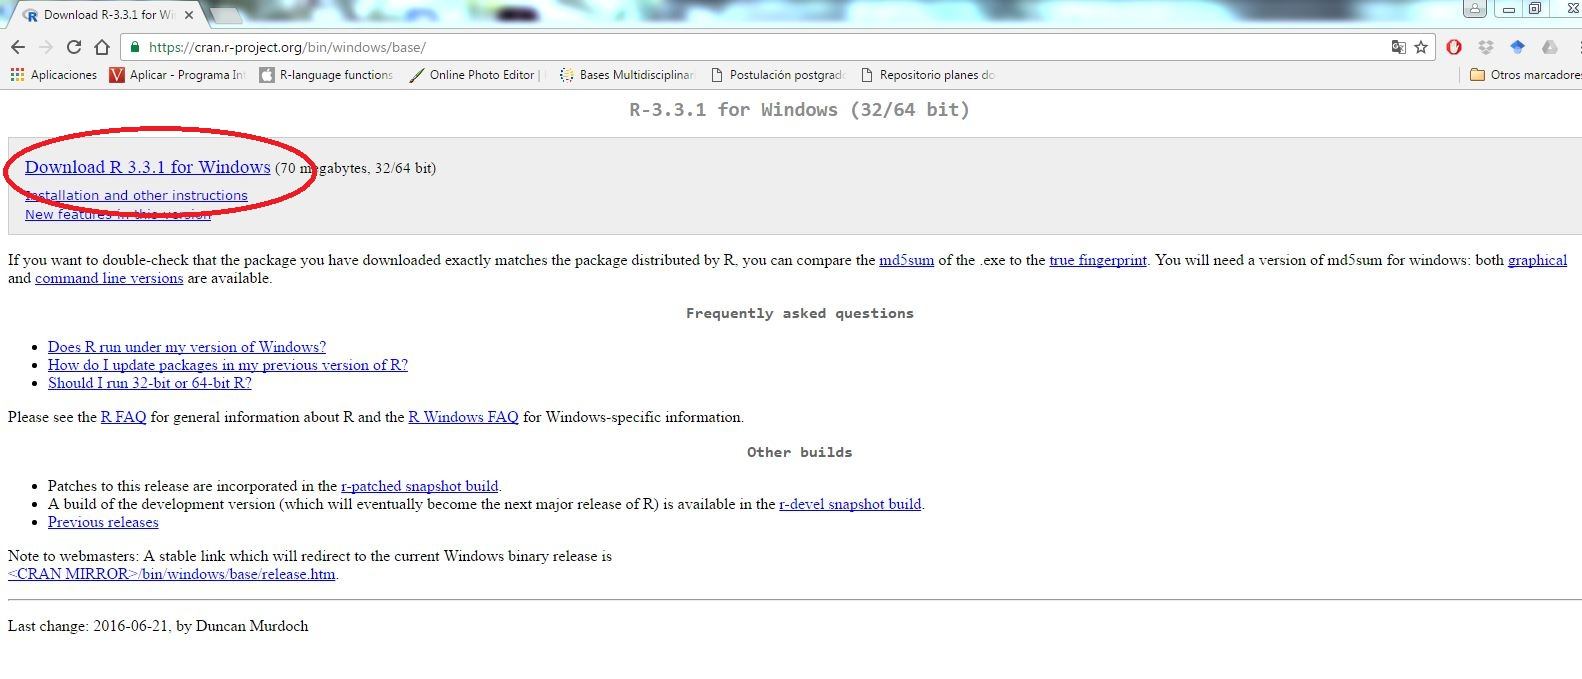
\includegraphics{imagen/descargarR.jpg}
\caption{Figura1. Descargando R}
\end{figure}

La instalación de \texttt{RStudio} es similar a R, debe ingresar en la
página de
\href{https://www.rstudio.com/products/rstudio/download/}{RStudio}. Una
vez en la página de descarga, seleccione la plataforma acorde a su
sistema operativo (Figura 2) y siga los pasos para terminar la
instalación.

\begin{figure}[htbp]
\centering
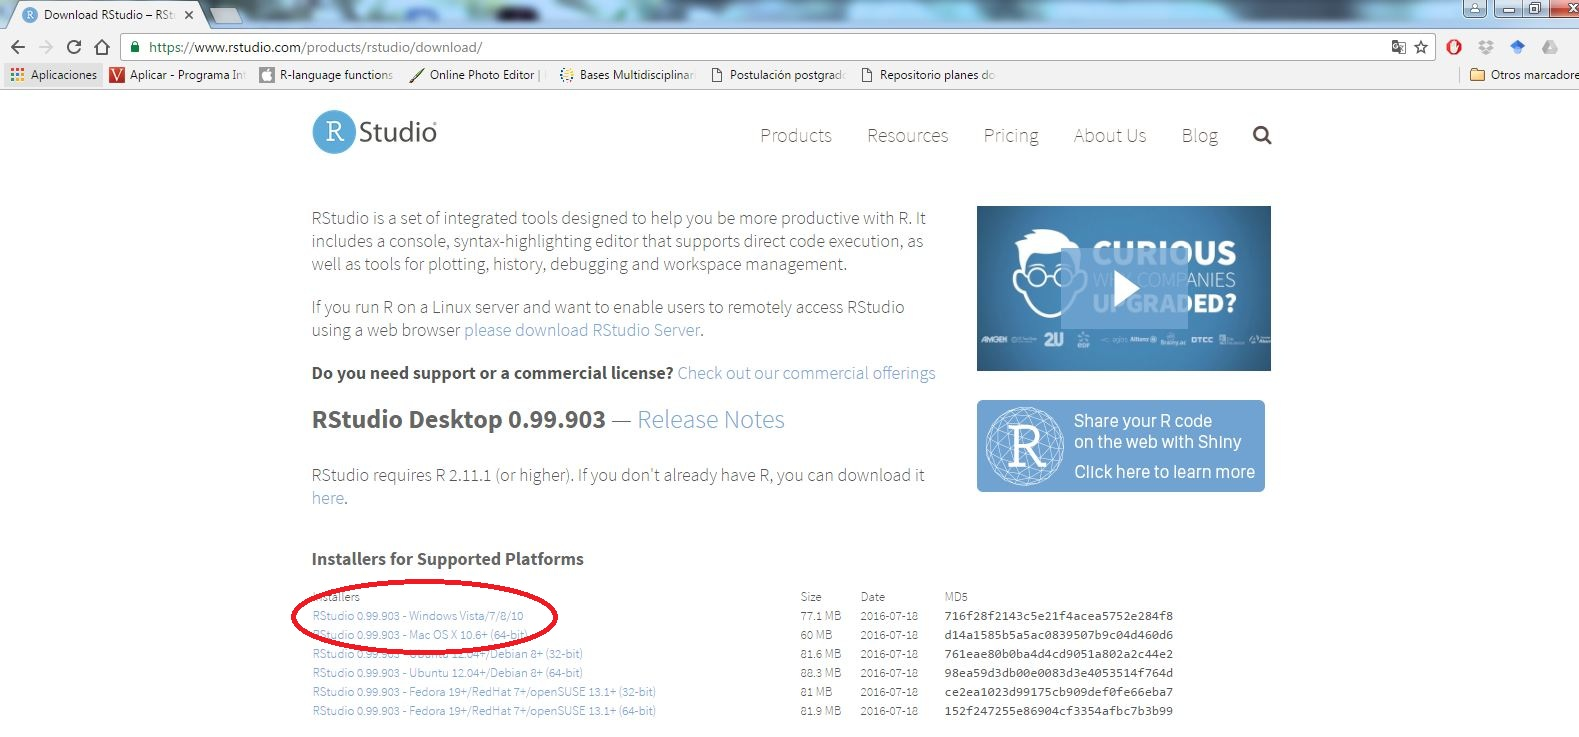
\includegraphics{imagen/descargarRStudio.jpg}
\caption{Figura2. Descargando RStudio}
\end{figure}

Una vez que hemos instalado R y RStudio podremos trabajar con los datos.
Una cosa importante es que RStudio no puede funcionar si no hemos
descargado R, así que se debe asegurar descargar los dos programas.
Trabajaremos en RStudio así que no es necesario que despliegue R.

\begin{quote}
Nota: ``El uso de comandos exige una curva de aprendizaje mayor que el
requerido por las interfaces gráficas, pero las ganancias en términos de
independencia, creatividad y control no son comparables. Escribir un
código supone una comprensión más profunda de aquello que se desea
aplicar'' (Elousa 2011).
\end{quote}

\begin{center}\rule{0.5\linewidth}{\linethickness}\end{center}

\section{Conozcamos RStudio antes de
empezar}\label{conozcamos-rstudio-antes-de-empezar}

\begin{figure}[htbp]
\centering
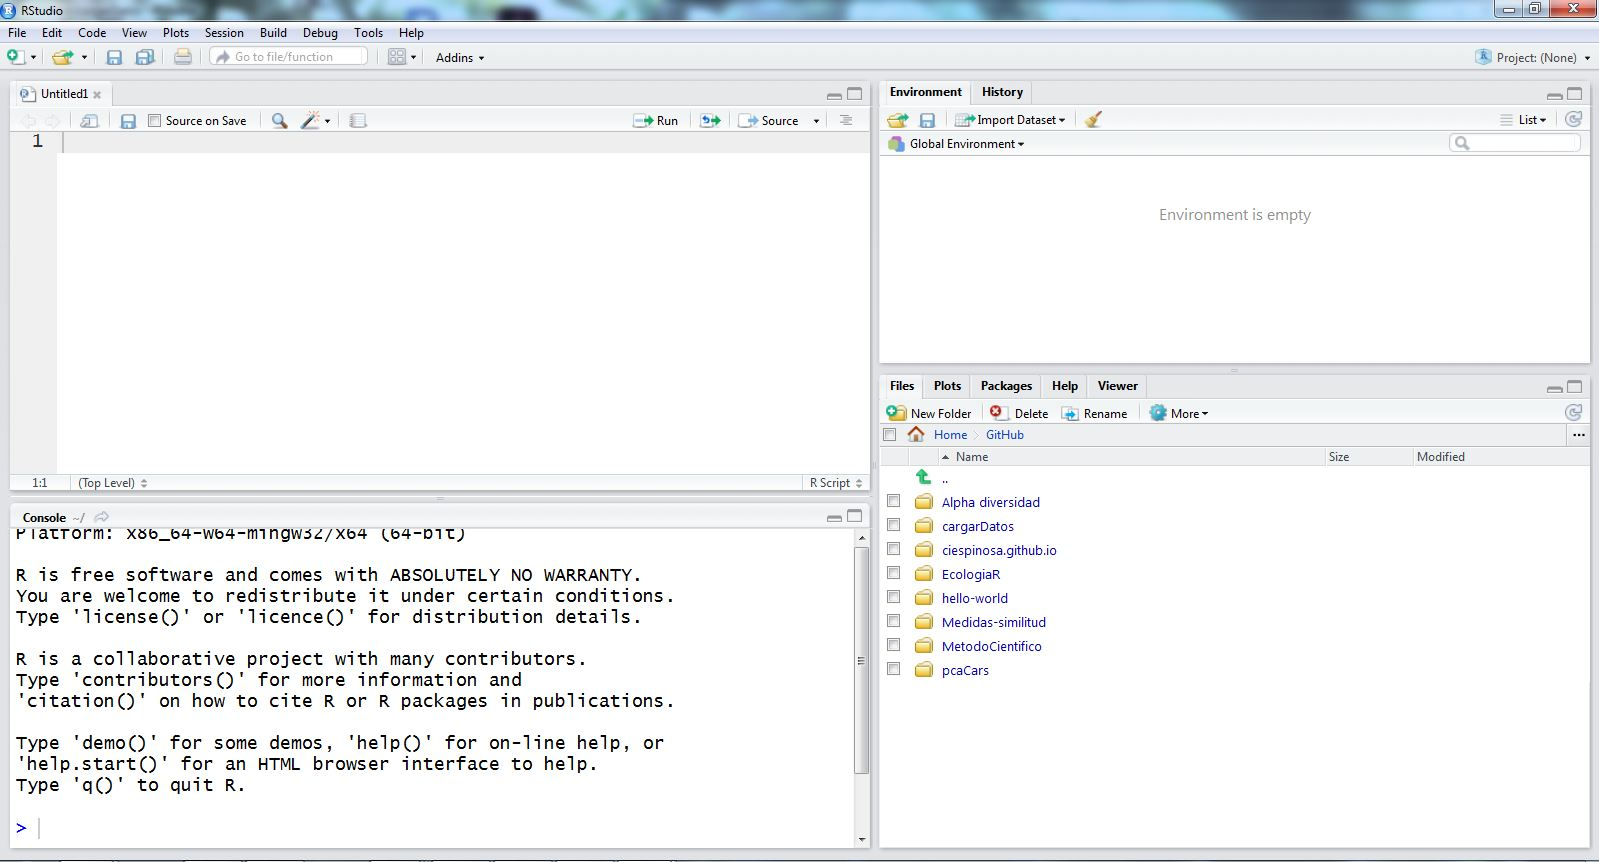
\includegraphics{imagen/RStudio.jpg}
\caption{Figura 4. Plataforma RStudio}
\end{figure}

Como vemos en la figura 4, RStudio está compuesto por cuatro ventanas.
Seguramente en su caso, si acaba de abrir RStudio le aparecerán
únicamente tres ventanas. A continuación, describiré cada una de las
ventanas.

La \textbf{primera ventana} (la que en su caso seguramente no tiene,
izquierda superior) lo constituye documentos que pueden ser de varios
tipos. El tipo básico es un documento con extensión \textbf{.R}, el cual
sirve para guardar el código desarrollado para el análisis. Vamos abrir
un documento .R (script), esto lo podemos hacer de al menos tres
maneras, la primera es ir al menú de la consola seleccionar
\texttt{File\ \textgreater{}\ New\ File\ \textgreater{}\ script}, la
segunda forma es seleccionar el icono del documento con una cruz verde

\includegraphics{imagen/RStudio_nuevo.jpg} y seleccionar
\texttt{R\ script}. La última opción es hacerlo desde el teclado,
presione \texttt{alt\ +\ shift} (mayúsculas) y la tecla \textbf{N}
obtendrá el mismo resultado.

Existen otros muchos archivos que podemos cargar, pero por ahora veremos
solo este.

La \textbf{segunda ventana} (derecha superior), esta ventana se verán
todos los objetos que iremos cargando o generando durante el trabajo en
RStudio, por ahora esta ventana estará vacía. Esta ventana nos muestra
la memoria activa de R, lo que en un computador se conoce como la
memoria RAM.

\begin{quote}
Vamos a generar algunos objetos y ver lo que pasa.
\end{quote}

\begin{Shaded}
\begin{Highlighting}[]
\NormalTok{nombre<-}\StringTok{ "Carlos Ivan"}
\NormalTok{apellido<-}\StringTok{ "Espinosa Iñiguez"}
\NormalTok{matriz<-}\StringTok{ }\KeywordTok{matrix}\NormalTok{(}\DecValTok{1}\NormalTok{:}\DecValTok{20}\NormalTok{, }\DecValTok{5}\NormalTok{,}\DecValTok{4}\NormalTok{)}
\end{Highlighting}
\end{Shaded}

Ahora podemos ver los objetos creados, algunos salen como valores y la
matriz sale como datos. Los objetos pueden ser abiertos para ver su
estructura. Si hacen clic en el nombre matriz verán que se abre una
nueva hoja en la primera ventana que corresponde a estos datos.

La \textbf{tercera columna} (izquierda abajo), corresponde a la consola
de R, esta es la consola donde se ejecutarán todos los códigos y se
realizarán los análisis. Esta ventana es R. RStudio incorpora a R dentro
de su ejecución, por lo que si no hemos instalado R esta ventana no
aparecerá.

La \textbf{cuarta columna} (derecha abajo), en esta ventana tenemos
varias pestañas. La primera \texttt{File} nos muestra todos los archivos
que están en la carpeta de mi proyecto, guardados en el disco duro.
Pueden ser archivos de datos, gráficos generados o el script de R que
estoy generando. La siguiente pestaña \texttt{Plots} mostrará los
gráficos que va ejecutando en R. La pestaña \texttt{Help} puede ser
usada para pedir ayuda de algún paquete o función que necesite usar, y
no esté claro de cómo hacerlo.

Bueno ya conocemos RStudio ahora si a trabajar.

\begin{quote}
Nota: El trabajar con códigos requiere que seamos ordenados y
sistemáticos, de no cumplir estos requerimientos tendrá un verdadero
dolor de cabeza. RStudio es una interesante plataforma que nos permite
organizar el trabajo. Siempre que inician un trabajo de análisis siga
los pasos propuestos a continuación.
\end{quote}

\begin{center}\rule{0.5\linewidth}{\linethickness}\end{center}

\section{Los primeros pasos}\label{los-primeros-pasos}

El trabajo de programación requiere ser ordenados, considero que
trabajar con RStudio nos ofrece algunas ventajas para organizar ese
trabajo.

\subsection{Primer Paso: Crear un
proyecto}\label{primer-paso-crear-un-proyecto}

Para crear un nuevo proyecto en RStudio debemos seguir los siguientes
pasos.

\begin{enumerate}
\def\labelenumi{\arabic{enumi}.}
\tightlist
\item
  Abrir RStudio
\item
  Hacer clic en \texttt{file} y seleccionar new \texttt{Project}
\item
  En la nueva ventana que se abrió, podemos seleccionar entre tres
  opciones, puesto que aún no estamos trabajando con versiones de
  control, por ahora podemos seleccionar entre nuevo directorio
  \texttt{New\ Directory} o un directorio existente
  \texttt{Existing\ Directory}.
\end{enumerate}

Si seleccionamos \texttt{New\ Directory}(nuevo directorio) se generará
una nueva carpeta en la ubicación que nosotros definamos, en esta
carpeta podremos poner todos los datos y demás información con la cual
trabajaremos. Cuando seleccionamos \texttt{Existing\ Directory} (un
directorio existente) RStudio generará un proyecto dentro de una carpeta
que ya exista en el computador. Por organización, siempre que estoy
iniciando un nuevo proyecto prefiero crear un nuevo directorio en el
cual colocaré únicamente los archivos que voy a utilizar en los
análisis.

\begin{enumerate}
\def\labelenumi{\arabic{enumi}.}
\setcounter{enumi}{3}
\item
  Si hemos elegido \texttt{New\ Directory} tendremos dos casilleros, el
  primero indica el nombre que le vamos a poner a la carpeta
  \texttt{Directory\ Name} y el segundo nos indica donde alojaremos esa
  carpeta \texttt{browse}.
\item
  Si hemos elegido \texttt{Existing\ Directory}, la siguiente ventana
  nos permite decir cuál es la carpeta que quiero enlazar. Hacer clic en
  \texttt{browse} buscar la carpeta donde colocaré el proyecto y
  aceptar.
\end{enumerate}

\subsection{Segundo Paso: Los códigos
usados}\label{segundo-paso-los-codigos-usados}

Si bien podemos trabajar directamente en la consola de R para ejecutar
los códigos, lo mejor es que desde el principio nos acostumbremos a
generar scripts, donde tengamos la información limpia y podamos saber lo
que estamos haciendo. Un Script es un archivo donde tendremos los
códigos de R, referenciados y organizados.

\textbf{Algunos consejos iniciales}

\begin{enumerate}
\def\labelenumi{\alph{enumi}.}
\item
  Todos los códigos que ponemos siempre deben ir acompañados de una nota
  que explique lo que están haciendo. La nota debe estar precedida por
  \textbf{\#}, con lo cual R no lee esta parte como código (Figura 4).
\item
  Recuerden siempre colocar sus archivos de datos en la carpeta del
  proyecto que generaron en el primer paso.
\item
  Si está probando cambios en el código, una vez que tiene un código que
  funciona, borre el código con error o que no le funcionó, tenga
  siempre su código limpio.
\item
  Una vez que escribe el código, este puede ser ejecutado desde la
  consola haciendo clic en la consola en el ícono run
  
\includegraphics{imagen/RStudio_Run.jpg} que se encuentra en la parte
  superior derecha de la ventana del script. Sin embargo, una mejor
  forma es tecleando \textbf{ctrl} y \textbf{enter}.
\item
  Cada vez que en el código iniciamos un nuevo tema, podemos poner un
  título seguido por cuatro guiones medios (- - - -), esto genera en
  RStudio una estructura de índice que puede ser navegada (Figura 5
  círculo rojo abajo a la izquierda).
\end{enumerate}

\begin{figure}[htbp]
\centering
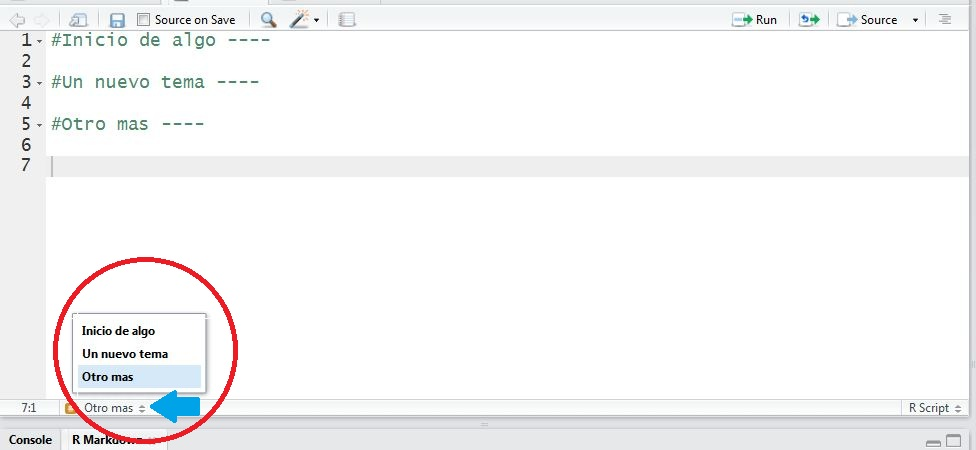
\includegraphics{imagen/estructura.jpg}
\caption{Figura 5. Estructura del script en RStudio}
\end{figure}

\begin{quote}
Nota: Es importante que sea organizado en la ejecución de los códigos,
siga los consejos y podrá mantener un código limpio y facil de acceder y
revisar.
\end{quote}

\begin{center}\rule{0.5\linewidth}{\linethickness}\end{center}

\section{El funcionamiento de R}\label{el-funcionamiento-de-r}

Hemos hablado mucho de \texttt{R} pero hasta ahora no hemos dicho que
es, ¿es un programa?, no, realmente no es un programa, es un entorno de
programación. R es considerado un dialecto del lenguaje \emph{S} el cual
fue desarrollado por los Laboratorios AT\&T Bell.

Aunque mucha gente se asusta cuando hablamos de R, como un lenguaje de
programación, la realidad es que R es un lenguaje bastante simple, está
orientado a \emph{Objetos}. Por otro lado, a diferencia de otros
lenguajes de programación los comandos escritos en el teclado, son
ejecutados directamente sin necesidad de construir ejecutables.

En R tenemos al menos tres grandes categorías de objetos; funciones,
datos y resultados. Cada una de estas tiene unas características
propias. Las \emph{funciones} normalmente se encuentran dentro de
paquetes, estos objetos traen comandos que permiten manipular los datos.
Accedemos a las funciones a través de comandos. Los \emph{datos} son
matrices o vectores de información los cuales son manipulados por las
funciones. Los \emph{resultados} son objetos resultantes de la
manipulación de los datos (Figura 3).

El funcionamiento de R se dá en la memoria activa, así que cada vez que
iniciamos a trabajar con R es necesario llamar los datos desde el disco
duro a la memoria activa. Para llamar paquetes (donde tenemos las
funciones) normalmente utilizamos la función \texttt{library}, mientras
que para llamar los datos utilizamos funciones como \texttt{read.table}.
Algunas veces nos interesa grabar un resultado desde la memoria activa
al disco duro para esto podemos utilizar funciones como
\texttt{write.table}. Finalmente, no todos los paquetes disponibles se
bajan cuando instalamos R, de hecho, solo se baja un paquete conocido
como paquete base. Cuando se necesita un nuevo paquete, este debe
llamarse desde internet, para ello utilizamos la función
\texttt{install.packages}. Existe un repositorio de todos los paquetes
disponibles (Comprehensive R Archive Network, \textbf{CRAN}) y varios
países tienen espejos de estos repositorios (espejos CRAN) a partir de
los cuales podemos descargar los paquetes.

\begin{quote}
Nota: Es muy importante que antes de empezar a trabajar con R seamos
conscientes de cómo funciona, esto facilitará entender lo que está
haciendo cuando introduce un código.
\end{quote}

\begin{center}\rule{0.5\linewidth}{\linethickness}\end{center}

\section{Los objetos}\label{los-objetos}

Como lo vimos en el apartado anterior, R opera sobre objetos y estos
objetos pueden ser diversos. Los diferentes tipos de objetos poseen unas
determinadas características de estructura, en el entorno R el tipo de
objeto se conoce como modo (mode) o clase (class).

Cuando estoy generado un objeto, es necesario darle una denominación, un
nombre, y asignarle a este unos datos. En R la función de asignación es
\texttt{\textless{}-}.

\begin{Shaded}
\begin{Highlighting}[]
\NormalTok{profe <-}\StringTok{ "Carlos Iván"}

\NormalTok{profe}
\end{Highlighting}
\end{Shaded}

\begin{verbatim}
## [1] "Carlos Iván"
\end{verbatim}

Hemos creado el objeto \emph{profe} asignando el nombre Carlos Iván. Si
ejecutamos el nombre del objeto R nos devuelve el contenido. Veamos otro
objeto.

\begin{Shaded}
\begin{Highlighting}[]
\NormalTok{Notas <-}\StringTok{ }\KeywordTok{c}\NormalTok{(}\KeywordTok{rep}\NormalTok{(}\DecValTok{10}\NormalTok{,}\DecValTok{5}\NormalTok{), }\KeywordTok{rep}\NormalTok{(}\DecValTok{7}\NormalTok{,}\DecValTok{3}\NormalTok{), }\KeywordTok{rep}\NormalTok{(}\FloatTok{8.5}\NormalTok{, }\DecValTok{12}\NormalTok{))}

\NormalTok{notas}

\CommentTok{#Error: object 'notas' not found}
\end{Highlighting}
\end{Shaded}

¿Qué es lo que sucedió?

Para R los nombres no son entendidos como palabras sino como una serie
de símbolos, por tanto la ``N'' no es lo mismo que la ``n'', por lo que
es necesario poner exactamente el nombre. En el caso del ejemplo, Notas
no es igual que notas. Volvamos a intentar.

\begin{Shaded}
\begin{Highlighting}[]
\NormalTok{Notas}
\end{Highlighting}
\end{Shaded}

\begin{verbatim}
##  [1] 10.0 10.0 10.0 10.0 10.0  7.0  7.0  7.0  8.5  8.5  8.5  8.5  8.5  8.5
## [15]  8.5  8.5  8.5  8.5  8.5  8.5
\end{verbatim}

Ahora si podemos ver que tenemos un curso muy aplicado.

\section{Operación de los objetos}\label{operacion-de-los-objetos}

A continuación, vamos a realizar un pequeño programa que nos ayude a
entender como los objetos pueden ser operados a través de comandos.
Haremos un seguimiento de los costos de un producto. Mi hija María Sol
tiene un pequeño negocio de chocolates, vamos a utilizar lo que ella
hace para ver lo potente que es R.

Para hacer los chocolates ella usa los siguientes ingredientes:

\begin{itemize}
\tightlist
\item
  Chocolate (Choco)
\item
  Nuez
\item
  Dulce de leche (D.leche)
\item
  Empaques (Empa)
\end{itemize}

Necesitamos saber cuál es el costo por chocolate y poder calcular una
ganancia.

\begin{Shaded}
\begin{Highlighting}[]
\NormalTok{Choco <-}\StringTok{ }\DecValTok{7} \CommentTok{#rinde 60 chocolates}
\NormalTok{Nuez <-}\StringTok{ }\FloatTok{2.5} \CommentTok{#rinde 40 chocolates}
\NormalTok{D.leche <-}\StringTok{ }\DecValTok{2} \CommentTok{#rinde 50 chocolates}
\NormalTok{Empa <-}\StringTok{ }\FloatTok{0.10} \CommentTok{#por cada chocolate}

\CommentTok{#¿Cuánto cuesta cada chocolate?}

\NormalTok{costo <-}\StringTok{ }\NormalTok{(Choco/}\DecValTok{60}\NormalTok{)+(Nuez/}\DecValTok{40}\NormalTok{)+(D.leche/}\DecValTok{50}\NormalTok{)+Empa}
\NormalTok{costo}
\end{Highlighting}
\end{Shaded}

\begin{verbatim}
## [1] 0.3191667
\end{verbatim}

\begin{Shaded}
\begin{Highlighting}[]
\CommentTok{#¿Cuanto debo sumar si quiero ganar el 30%?}

\NormalTok{ganancia <-}\StringTok{ }\NormalTok{costo*}\FloatTok{0.3}
\NormalTok{ganancia}
\end{Highlighting}
\end{Shaded}

\begin{verbatim}
## [1] 0.09575
\end{verbatim}

\begin{Shaded}
\begin{Highlighting}[]
\CommentTok{#¿Cuánto cuesta cada chocolate?}

\NormalTok{pvp<-}\StringTok{ }\NormalTok{costo+ganancia}
\NormalTok{pvp}
\end{Highlighting}
\end{Shaded}

\begin{verbatim}
## [1] 0.4149167
\end{verbatim}

\begin{Shaded}
\begin{Highlighting}[]
\CommentTok{#¿Cuantos chocolates debo vender si quiero ganar 100 USD mensuales?}

\NormalTok{venta<-}\StringTok{ }\DecValTok{100}\NormalTok{/ganancia}
\NormalTok{venta}
\end{Highlighting}
\end{Shaded}

\begin{verbatim}
## [1] 1044.386
\end{verbatim}

Como esto puede ser engorroso podríamos desarrollar una función que
calcule cada uno de estas mediciones.

\begin{Shaded}
\begin{Highlighting}[]
\NormalTok{negocio <-}\StringTok{ }\NormalTok{function(C,N,D,E,G)\{}
  \NormalTok{x <-}\StringTok{ }\NormalTok{(C/}\DecValTok{60}\NormalTok{)+(N/}\DecValTok{40}\NormalTok{)+(D/}\DecValTok{50}\NormalTok{)+E}
  \NormalTok{y <-}\StringTok{ }\NormalTok{x*G}
  \NormalTok{z <-}\StringTok{ }\NormalTok{x+y}
  
  \NormalTok{neg <-}\StringTok{ }\KeywordTok{c}\NormalTok{(x,y,z)}
  \KeywordTok{names}\NormalTok{(neg) <-}\StringTok{ }\KeywordTok{c}\NormalTok{(}\StringTok{"costo"}\NormalTok{, }\StringTok{"ganancia"}\NormalTok{, }\StringTok{"PVP"}\NormalTok{)}
  \KeywordTok{return}\NormalTok{(neg)}
\NormalTok{\}}

\CommentTok{#Veamos cuanto cuesta el chocolate}

\KeywordTok{negocio}\NormalTok{(}\DataTypeTok{C=}\DecValTok{7}\NormalTok{,}\DataTypeTok{N=}\DecValTok{25}\NormalTok{,}\DataTypeTok{D=}\DecValTok{2}\NormalTok{,}\DataTypeTok{E=}\FloatTok{0.10}\NormalTok{, }\DataTypeTok{G=}\FloatTok{0.3}\NormalTok{)}
\end{Highlighting}
\end{Shaded}

\begin{verbatim}
##     costo  ganancia       PVP 
## 0.8816667 0.2645000 1.1461667
\end{verbatim}

\begin{Shaded}
\begin{Highlighting}[]
\CommentTok{#Ahora puede cambiar el costo de cualquiera de }
\CommentTok{#los elementos y tendrá automáticamente los parámetros}
\CommentTok{#de su negocio}
\end{Highlighting}
\end{Shaded}

Como ven R es muy potente y podemos hacer muchas cosas con el, cada uno
de los objetos pueden ser operados, en este caso a los objetos los hemos
multiplicado, dividido o sumado. Verán más adelante que las operaciones
pueden ser mucho más complejas.

\begin{center}\rule{0.5\linewidth}{\linethickness}\end{center}

\subsection{Tipos de Objetos}\label{tipos-de-objetos}

Los objetos pueden tener varios tipos (typeof) y estos se diferencian
por el tipo de datos (elementos) por los que están conformados. Los
objetos más comunes son los objetos dobles, enteros, lógicos y carácter.

Veamos un ejemplo de este tipo de objetos.

\begin{Shaded}
\begin{Highlighting}[]
\NormalTok{d <-}\StringTok{ }\FloatTok{3.5}
\NormalTok{e <-}\StringTok{ }\NormalTok{8L}
\NormalTok{l <-}\StringTok{ }\NormalTok{e>d}
\NormalTok{c <-}\StringTok{ "a"}

\NormalTok{d;e;l;c}
\end{Highlighting}
\end{Shaded}

\begin{verbatim}
## [1] 3.5
\end{verbatim}

\begin{verbatim}
## [1] 8
\end{verbatim}

\begin{verbatim}
## [1] TRUE
\end{verbatim}

\begin{verbatim}
## [1] "a"
\end{verbatim}

Podemos preguntar a R el tipo de objeto con el que estamos trabajando,
para esto utilizamos las funciones \emph{is.double, is.integer,
is.logical, is.character}

\begin{Shaded}
\begin{Highlighting}[]
\KeywordTok{is.double}\NormalTok{(d); }\KeywordTok{is.double}\NormalTok{(e); }\KeywordTok{is.double}\NormalTok{(l)}
\end{Highlighting}
\end{Shaded}

\begin{verbatim}
## [1] TRUE
\end{verbatim}

\begin{verbatim}
## [1] FALSE
\end{verbatim}

\begin{verbatim}
## [1] FALSE
\end{verbatim}

\begin{Shaded}
\begin{Highlighting}[]
\KeywordTok{is.integer}\NormalTok{(d); }\KeywordTok{is.integer}\NormalTok{(e); }\KeywordTok{is.integer}\NormalTok{(l)}
\end{Highlighting}
\end{Shaded}

\begin{verbatim}
## [1] FALSE
\end{verbatim}

\begin{verbatim}
## [1] TRUE
\end{verbatim}

\begin{verbatim}
## [1] FALSE
\end{verbatim}

\begin{Shaded}
\begin{Highlighting}[]
\KeywordTok{is.logical}\NormalTok{(d); }\KeywordTok{is.logical}\NormalTok{(l); }\KeywordTok{is.logical}\NormalTok{(c)}
\end{Highlighting}
\end{Shaded}

\begin{verbatim}
## [1] FALSE
\end{verbatim}

\begin{verbatim}
## [1] TRUE
\end{verbatim}

\begin{verbatim}
## [1] FALSE
\end{verbatim}

\begin{Shaded}
\begin{Highlighting}[]
\KeywordTok{is.character}\NormalTok{(d); }\KeywordTok{is.character}\NormalTok{(l); }\KeywordTok{is.character}\NormalTok{(c)}
\end{Highlighting}
\end{Shaded}

\begin{verbatim}
## [1] FALSE
\end{verbatim}

\begin{verbatim}
## [1] FALSE
\end{verbatim}

\begin{verbatim}
## [1] TRUE
\end{verbatim}

Como vemos cada uno de estos objetos son diferentes. Los objetos dobles
(double) están formados por datos continuos, mientras que los enteros
(integer) están formados por datos de tipo conteo. Finalmente, los
objetos lógicos se dan luego de una operación lógica. Podemos preguntar
directamente el tipo de datos que tiene el objeto con la función
\emph{typeof}

\begin{Shaded}
\begin{Highlighting}[]
\KeywordTok{typeof}\NormalTok{(d); }\KeywordTok{typeof}\NormalTok{(l); }\KeywordTok{typeof}\NormalTok{(c)}
\end{Highlighting}
\end{Shaded}

\begin{verbatim}
## [1] "double"
\end{verbatim}

\begin{verbatim}
## [1] "logical"
\end{verbatim}

\begin{verbatim}
## [1] "character"
\end{verbatim}

\subsection{Estructura de los objetos}\label{estructura-de-los-objetos}

La estructura de los objetos en R puede ser descrita en base de su
dimensionalidad y en base a su constitución. Los objetos pueden tener
una, dos o n dimensiones, y pueden ser homogéneos o heterogéneos en
cuanto al tipo de elementos que lo constituyen. Como vemos en la
siguiente tabla, en función de estas dos características podemos tener
algunos tipos de estructuras de los objetos.

\begin{verbatim}
## Warning: package 'knitr' was built under R version 3.5.3
\end{verbatim}

\begin{longtable}[]{@{}lll@{}}
\caption{Estructura de objetos. Fuente: Wickham, 2014}\tabularnewline
\toprule
& Homogéneos & Heterogéneos\tabularnewline
\midrule
\endfirsthead
\toprule
& Homogéneos & Heterogéneos\tabularnewline
\midrule
\endhead
1d & Atomic vector & List\tabularnewline
2d & Matrix & Data frame\tabularnewline
nd & Array &\tabularnewline
\bottomrule
\end{longtable}

Ahora vamos a ver en detalle cada uno de los objetos.

\subsubsection{Vectores (Vectors)}\label{vectores-vectors}

Los vectores son las estructuras más simples de R. Los vectores tienen
una sola dimensión, y los elementos que lo constituyen definen el tipo
de vector que es, así, si es un vector con números enteros será un
vector numérico (integrer), o un vector con letras será un vector de
carácter (character). El vector puede ser desde un solo valor hasta
varios miles, pero debe estar constituido por un solo tipo de elemento.

Veamos algunos ejemplos de vectores.

\begin{Shaded}
\begin{Highlighting}[]
\NormalTok{a <-}\StringTok{ }\DecValTok{5}\NormalTok{:}\DecValTok{12} \CommentTok{#vector numérico}
\NormalTok{b <-}\StringTok{ }\NormalTok{a>=}\DecValTok{6}\NormalTok{&a<=}\DecValTok{10} \CommentTok{#vector lógico}
\NormalTok{c <-}\StringTok{ }\KeywordTok{c}\NormalTok{(letters[}\DecValTok{1}\NormalTok{:}\DecValTok{10}\NormalTok{]) }\CommentTok{#vector de carácter}

\NormalTok{a;b;c}
\end{Highlighting}
\end{Shaded}

\begin{verbatim}
## [1]  5  6  7  8  9 10 11 12
\end{verbatim}

\begin{verbatim}
## [1] FALSE  TRUE  TRUE  TRUE  TRUE  TRUE FALSE FALSE
\end{verbatim}

\begin{verbatim}
##  [1] "a" "b" "c" "d" "e" "f" "g" "h" "i" "j"
\end{verbatim}

Cada uno de estos vectores fue generado utilizando diferentes funciones
o códigos. El vector numérico se generó utilizando únicamente una
secuencia de datos entre 5 y 12, lo hicimos utilizando los dos puntos,
esto nos sirve cuando queremos una secuencia ininterrumpida entre dos
números, sin embargo, si queremos tener secuencias con diferentes
distancias. Para el vector lógico hemos utilizado operadores lógicos
como \textbf{igual o mayor que (\textgreater{}=)}, \textbf{menor o igual
que (\textless{}=)} , \textbf{y (\&)}. Finalmente, para generar un
vector de carácter hemos utilizado la función \textbf{concatenación
(\emph{c})}, esta función permite encadenar varios componentes en un
vector.

Veamos el tipo de vector que hemos generado.

\begin{Shaded}
\begin{Highlighting}[]
\KeywordTok{mode}\NormalTok{(a);}\KeywordTok{mode}\NormalTok{(b);}\KeywordTok{mode}\NormalTok{(c)}
\end{Highlighting}
\end{Shaded}

\begin{verbatim}
## [1] "numeric"
\end{verbatim}

\begin{verbatim}
## [1] "logical"
\end{verbatim}

\begin{verbatim}
## [1] "character"
\end{verbatim}

Como comentamos los vectores lógicos son generados a partir de
expresiones lógicas (en la tabla 1 se pueden ver algunos operadores
lógicos).

\textbf{Tabla 1}: Operadores Lógicos

\begin{longtable}[]{@{}ll@{}}
\toprule
\begin{minipage}[b]{0.29\columnwidth}\raggedright\strut
Descripción\strut
\end{minipage} & \begin{minipage}[b]{0.17\columnwidth}\raggedright\strut
Operadores\strut
\end{minipage}\tabularnewline
\midrule
\endhead
\begin{minipage}[t]{0.29\columnwidth}\raggedright\strut
Mayor que\strut
\end{minipage} & \begin{minipage}[t]{0.17\columnwidth}\raggedright\strut
\(>\)\strut
\end{minipage}\tabularnewline
\begin{minipage}[t]{0.29\columnwidth}\raggedright\strut
Menor que\strut
\end{minipage} & \begin{minipage}[t]{0.17\columnwidth}\raggedright\strut
\(<\)\strut
\end{minipage}\tabularnewline
\begin{minipage}[t]{0.29\columnwidth}\raggedright\strut
Mayor o igual que\strut
\end{minipage} & \begin{minipage}[t]{0.17\columnwidth}\raggedright\strut
\(>=\)\strut
\end{minipage}\tabularnewline
\begin{minipage}[t]{0.29\columnwidth}\raggedright\strut
Menor o igual que\strut
\end{minipage} & \begin{minipage}[t]{0.17\columnwidth}\raggedright\strut
\(<=\)\strut
\end{minipage}\tabularnewline
\begin{minipage}[t]{0.29\columnwidth}\raggedright\strut
Igual que\strut
\end{minipage} & \begin{minipage}[t]{0.17\columnwidth}\raggedright\strut
\(==\)\strut
\end{minipage}\tabularnewline
\begin{minipage}[t]{0.29\columnwidth}\raggedright\strut
No es igual que\strut
\end{minipage} & \begin{minipage}[t]{0.17\columnwidth}\raggedright\strut
\(!=\)\strut
\end{minipage}\tabularnewline
\bottomrule
\end{longtable}

En el caso de los vectores numéricos y categóricos hemos utilizado
secuencia y concatenar, pero podríamos utilizar algunas otras funciones.

\begin{Shaded}
\begin{Highlighting}[]
\NormalTok{secA<-}\StringTok{ }\KeywordTok{seq}\NormalTok{(}\DataTypeTok{from=}\DecValTok{10}\NormalTok{, }\DataTypeTok{to=}\DecValTok{290}\NormalTok{, }\DataTypeTok{by=}\DecValTok{20}\NormalTok{)}
\NormalTok{secA}
\end{Highlighting}
\end{Shaded}

\begin{verbatim}
##  [1]  10  30  50  70  90 110 130 150 170 190 210 230 250 270 290
\end{verbatim}

Aquí hemos utilizado la secuencia entre 10 y 290, pero le hemos dicho
que lo haga cada 20 unidades. R entiende el orden de los datos
proporcionados, así que la expresión que acabamos de ejecutar es
exactamente igual a: \texttt{secA\textless{}-\ seq(10,\ 290,\ 20)}

Otra de las funciones que se ocupan mucho para la generación de los
vectores es la función \texttt{rep}. Esta función permite repetir varias
veces un argumento.

\begin{Shaded}
\begin{Highlighting}[]
\NormalTok{repA <-}\StringTok{ }\KeywordTok{rep}\NormalTok{(}\DecValTok{1}\NormalTok{:}\DecValTok{5}\NormalTok{, }\DecValTok{3}\NormalTok{) }\CommentTok{#Repite la secuencia de uno a cinco, tres veces }

\NormalTok{repB <-}\StringTok{ }\KeywordTok{rep} \NormalTok{(}\DecValTok{1}\NormalTok{:}\DecValTok{5}\NormalTok{, }\KeywordTok{c}\NormalTok{(}\DecValTok{3}\NormalTok{,}\DecValTok{2}\NormalTok{,}\DecValTok{7}\NormalTok{,}\DecValTok{2}\NormalTok{,}\DecValTok{8}\NormalTok{)) }\CommentTok{#Repite para cada número de la secuencia las veces indicada por el vector de repetición.}

\NormalTok{repC <-}\StringTok{ }\KeywordTok{rep}\NormalTok{(letters[}\DecValTok{1}\NormalTok{:}\DecValTok{3}\NormalTok{], }\DecValTok{3}\NormalTok{) }\CommentTok{#Repite las letras de uno a tres, tres veces}

\NormalTok{repA; repB; repC}
\end{Highlighting}
\end{Shaded}

\begin{verbatim}
##  [1] 1 2 3 4 5 1 2 3 4 5 1 2 3 4 5
\end{verbatim}

\begin{verbatim}
##  [1] 1 1 1 2 2 3 3 3 3 3 3 3 4 4 5 5 5 5 5 5 5 5
\end{verbatim}

\begin{verbatim}
## [1] "a" "b" "c" "a" "b" "c" "a" "b" "c"
\end{verbatim}

Podemos generar un vector de carácter al combinar letras y números en un
vector, para esto utilizamos la función \texttt{paste}.

\begin{Shaded}
\begin{Highlighting}[]
\NormalTok{pasA <-}\StringTok{ }\KeywordTok{paste}\NormalTok{(LETTERS[}\DecValTok{8}\NormalTok{:}\DecValTok{16}\NormalTok{], }\DecValTok{1}\NormalTok{:}\DecValTok{8}\NormalTok{, }\DataTypeTok{sep=}\StringTok{"_"}\NormalTok{)}

\CommentTok{#Algo más complicado}

\NormalTok{pasB <-}\StringTok{ }\KeywordTok{paste}\NormalTok{(letters[}\DecValTok{1}\NormalTok{:}\DecValTok{9}\NormalTok{], }\KeywordTok{rep}\NormalTok{(}\DecValTok{1}\NormalTok{:}\DecValTok{3}\NormalTok{, }\DecValTok{3}\NormalTok{), }\DataTypeTok{sep=}\StringTok{"a"} \NormalTok{)}

\NormalTok{pasA; pasB}
\end{Highlighting}
\end{Shaded}

\begin{verbatim}
## [1] "H_1" "I_2" "J_3" "K_4" "L_5" "M_6" "N_7" "O_8" "P_1"
\end{verbatim}

\begin{verbatim}
## [1] "aa1" "ba2" "ca3" "da1" "ea2" "fa3" "ga1" "ha2" "ia3"
\end{verbatim}

La función \emph{paste} requiere tres argumentos; los dos vectores que
serán unidos y un símbolo de separación.

Como vemos los vectores deben estar compuestos por un solo tipo de
elementos, si un vector tiene más de un tipo de elemento estos son
\texttt{coaccionados} al tipo más flexible. De esta forma en un vector
que tenga números y una letra, estos pueden ser coaccionados (coerced) a
caracteres.

\begin{Shaded}
\begin{Highlighting}[]
\NormalTok{a <-}\StringTok{ }\KeywordTok{c}\NormalTok{(}\DecValTok{2}\NormalTok{,}\DecValTok{5}\NormalTok{,}\DecValTok{7}\NormalTok{,}\DecValTok{5}\NormalTok{,}\DecValTok{3}\NormalTok{, }\DecValTok{7}\NormalTok{, }\StringTok{"a"}\NormalTok{)}
\KeywordTok{typeof}\NormalTok{(a)}
\end{Highlighting}
\end{Shaded}

\begin{verbatim}
## [1] "character"
\end{verbatim}

\begin{Shaded}
\begin{Highlighting}[]
\NormalTok{a}
\end{Highlighting}
\end{Shaded}

\begin{verbatim}
## [1] "2" "5" "7" "5" "3" "7" "a"
\end{verbatim}

Como vemos este vector fue convertido en un vector tipo carácter. Los
vectores lógicos son coaccionado a 0 y 1, falso y verdadero
respectivamente.

\begin{Shaded}
\begin{Highlighting}[]
\NormalTok{al <-}\StringTok{ }\NormalTok{a==}\StringTok{"a"}
\NormalTok{al}
\end{Highlighting}
\end{Shaded}

\begin{verbatim}
## [1] FALSE FALSE FALSE FALSE FALSE FALSE  TRUE
\end{verbatim}

\begin{Shaded}
\begin{Highlighting}[]
\KeywordTok{sum}\NormalTok{(al)}
\end{Highlighting}
\end{Shaded}

\begin{verbatim}
## [1] 1
\end{verbatim}

Podemos forzar una coerción usando la función \texttt{as.numeric} por
ejemplo, para cambiar unos factores a números. Usaremos
\texttt{as.character} para convertir un vector a caracteres, o
\texttt{as.matrix} para convertir un data frame en una matriz.

\subsubsection{Factores (Factors)}\label{factores-factors}

Los factores es un modo sencillo en que se guardan las variables
categóricas. Si tenemos un vector con 50 hombres y 50 mujeres, si el
vector se encuentra como factor, en vez de tener 100 datos lo que tengo
es hombres 50 y mujeres 50. Cada categoría se repite una cierta cantidad
de veces.

\begin{Shaded}
\begin{Highlighting}[]
\NormalTok{cat <-}\StringTok{ }\KeywordTok{rep}\NormalTok{(}\KeywordTok{c}\NormalTok{(}\StringTok{"alto"}\NormalTok{, }\StringTok{"medio"}\NormalTok{, }\StringTok{"bajo"}\NormalTok{), }\KeywordTok{c}\NormalTok{(}\DecValTok{10}\NormalTok{, }\DecValTok{20}\NormalTok{,}\DecValTok{25}\NormalTok{))}

\NormalTok{cat <-}\StringTok{ }\KeywordTok{factor}\NormalTok{(cat) }

\KeywordTok{levels}\NormalTok{(cat)}
\end{Highlighting}
\end{Shaded}

\begin{verbatim}
## [1] "alto"  "bajo"  "medio"
\end{verbatim}

La función \texttt{factor} nos permite convertir el vector de caracteres
en un vector factor. Ejecute la primera línea de código y luego el
nombre de este objeto, ahora ejecute la segunda línea y luego el nombre
del objeto. ¿Cuál es la diferencia?

Efectivamente cuando ejecuta la segunda línea al final aparece una
observación: \texttt{Levels:\ alto\ bajo\ medio}

Como vemos los niveles (levels) son mostrados en base a un orden
alfanúmerico, este orden será el utilizado para los gráficos y los
análisis por lo que es importante saber si este orden es el que
queremos. Si no es así podemos utilizar la función \texttt{relevel} para
decir cuál es el nivel que queremos que salga primero, o en la función
factor informar el orden de los niveles.

\begin{Shaded}
\begin{Highlighting}[]
\NormalTok{cat1 <-}\StringTok{ }\KeywordTok{relevel}\NormalTok{(cat, }\DataTypeTok{ref =} \StringTok{"bajo"}\NormalTok{)}

\NormalTok{cat2 <-}\StringTok{ }\KeywordTok{factor}\NormalTok{(cat, }\DataTypeTok{levels =} \KeywordTok{c}\NormalTok{(}\StringTok{"bajo"}\NormalTok{, }\StringTok{"medio"}\NormalTok{, }\StringTok{"alto"}\NormalTok{))}

\NormalTok{cat1; cat2}
\end{Highlighting}
\end{Shaded}

\begin{verbatim}
##  [1] alto  alto  alto  alto  alto  alto  alto  alto  alto  alto  medio
## [12] medio medio medio medio medio medio medio medio medio medio medio
## [23] medio medio medio medio medio medio medio medio bajo  bajo  bajo 
## [34] bajo  bajo  bajo  bajo  bajo  bajo  bajo  bajo  bajo  bajo  bajo 
## [45] bajo  bajo  bajo  bajo  bajo  bajo  bajo  bajo  bajo  bajo  bajo 
## Levels: bajo alto medio
\end{verbatim}

\begin{verbatim}
##  [1] alto  alto  alto  alto  alto  alto  alto  alto  alto  alto  medio
## [12] medio medio medio medio medio medio medio medio medio medio medio
## [23] medio medio medio medio medio medio medio medio bajo  bajo  bajo 
## [34] bajo  bajo  bajo  bajo  bajo  bajo  bajo  bajo  bajo  bajo  bajo 
## [45] bajo  bajo  bajo  bajo  bajo  bajo  bajo  bajo  bajo  bajo  bajo 
## Levels: bajo medio alto
\end{verbatim}

Podemos también unificar niveles, reduciendo la cantidad de niveles
resultantes. Vamos a unificar los niveles alto y medio en un nivel
llamado \emph{contaminado} y el bajo lo vamos a llamar \emph{no
contaminado}.

\begin{Shaded}
\begin{Highlighting}[]
\NormalTok{cat3 <-}\StringTok{ }\NormalTok{cat}
\KeywordTok{levels}\NormalTok{(cat3) <-}\StringTok{ }\KeywordTok{list}\NormalTok{(}\DataTypeTok{no.contaminado =} \StringTok{"bajo"}\NormalTok{, }\DataTypeTok{contaminado=} \KeywordTok{c}\NormalTok{(}\StringTok{"medio"}\NormalTok{, }\StringTok{"alto"}\NormalTok{))}
\NormalTok{cat3}
\end{Highlighting}
\end{Shaded}

\begin{verbatim}
##  [1] contaminado    contaminado    contaminado    contaminado   
##  [5] contaminado    contaminado    contaminado    contaminado   
##  [9] contaminado    contaminado    contaminado    contaminado   
## [13] contaminado    contaminado    contaminado    contaminado   
## [17] contaminado    contaminado    contaminado    contaminado   
## [21] contaminado    contaminado    contaminado    contaminado   
## [25] contaminado    contaminado    contaminado    contaminado   
## [29] contaminado    contaminado    no.contaminado no.contaminado
## [33] no.contaminado no.contaminado no.contaminado no.contaminado
## [37] no.contaminado no.contaminado no.contaminado no.contaminado
## [41] no.contaminado no.contaminado no.contaminado no.contaminado
## [45] no.contaminado no.contaminado no.contaminado no.contaminado
## [49] no.contaminado no.contaminado no.contaminado no.contaminado
## [53] no.contaminado no.contaminado no.contaminado
## Levels: no.contaminado contaminado
\end{verbatim}

Muy bien lo que hemos hecho es transformar los niveles iniciales a dos
nuevos niveles. Muchas veces cuando trabajamos con datos nos interesa
hacer lo contrario, los datos numéricos transformarlos a categorias.
Esto lo podemos hacer con la función \emph{cut()}.

\begin{Shaded}
\begin{Highlighting}[]
\NormalTok{x <-}\StringTok{ }\DecValTok{1}\NormalTok{:}\DecValTok{100} \CommentTok{# Porcentaje de contaminación}

\NormalTok{xcat <-}\StringTok{ }\KeywordTok{cut}\NormalTok{(x, }\DataTypeTok{breaks =} \KeywordTok{c}\NormalTok{(}\DecValTok{0}\NormalTok{, }\DecValTok{30}\NormalTok{, }\DecValTok{70}\NormalTok{, }\DecValTok{100}\NormalTok{))}
\NormalTok{xcat1 <-}\StringTok{ }\KeywordTok{cut}\NormalTok{(x, }\DataTypeTok{breaks =} \KeywordTok{c}\NormalTok{(}\DecValTok{0}\NormalTok{, }\DecValTok{30}\NormalTok{, }\DecValTok{70}\NormalTok{, }\DecValTok{100}\NormalTok{), }\DataTypeTok{labels=}\KeywordTok{c}\NormalTok{(}\StringTok{"bajo"}\NormalTok{, }\StringTok{"medio"}\NormalTok{, }\StringTok{"alto"}\NormalTok{))}
\end{Highlighting}
\end{Shaded}

Lo que hemos hecho es generar tres niveles; el primero entre 0 y 30, el
segundo entre 30 y 70 y el tercero entre 70 y 100. En xcat1 hemos
asignado unos nombres a cada una de las nuebas categorias con el
argumento \emph{labels}.

\subsubsection{Listas}\label{listas}

Una lista es una colección ordenada de elementos de distinto tipo. Una
lista puede contener otra lista, y de este modo puede utilizarse para
construir estructuras de datos arbitrarias. Las listas son utilizadas
por R como salidas de las funciones estadísticas.

Las listas al igual que los vectores tienen una sola dimensión, pero a
diferencia de los vectores estas pueden estar compuestas por diferentes
tipos de elementos.

\begin{Shaded}
\begin{Highlighting}[]
\NormalTok{listA <-}\StringTok{ }\KeywordTok{list}\NormalTok{(}\StringTok{"a"}\NormalTok{, }\StringTok{"b"}\NormalTok{, }\KeywordTok{c}\NormalTok{(}\DecValTok{1}\NormalTok{))}
\NormalTok{listA}
\end{Highlighting}
\end{Shaded}

\begin{verbatim}
## [[1]]
## [1] "a"
## 
## [[2]]
## [1] "b"
## 
## [[3]]
## [1] 1
\end{verbatim}

Como vemos las listas pueden tener una estructura lineal, pero puede
estar compuesta por diversos elementos. Incluso la lista puede incluir
listas, así se puede generar una estructura de datos jerarquizada.

\begin{Shaded}
\begin{Highlighting}[]
\NormalTok{listA <-}\StringTok{ }\KeywordTok{list}\NormalTok{(}\DecValTok{1}\NormalTok{:}\DecValTok{5}\NormalTok{, }\KeywordTok{list}\NormalTok{(}\KeywordTok{rep}\NormalTok{(}\DecValTok{1}\NormalTok{,}\DecValTok{3}\NormalTok{)), }\KeywordTok{list}\NormalTok{(}\StringTok{"a"}\NormalTok{, }\StringTok{"b"}\NormalTok{, }\StringTok{"c"}\NormalTok{, }\KeywordTok{list}\NormalTok{(}\KeywordTok{rep}\NormalTok{(}\StringTok{"a"}\NormalTok{,}\DecValTok{3}\NormalTok{))))}
\KeywordTok{str}\NormalTok{(listA)}
\end{Highlighting}
\end{Shaded}

\begin{verbatim}
## List of 3
##  $ : int [1:5] 1 2 3 4 5
##  $ :List of 1
##   ..$ : num [1:3] 1 1 1
##  $ :List of 4
##   ..$ : chr "a"
##   ..$ : chr "b"
##   ..$ : chr "c"
##   ..$ :List of 1
##   .. ..$ : chr [1:3] "a" "a" "a"
\end{verbatim}

Para convertir la lista en un vector podemos usar la función
\texttt{unlist}, lo que vuelve la lista a un vector. Si esta lista
contiene elementos de diferente tipo los elementos serán coaccionados.

\begin{Shaded}
\begin{Highlighting}[]
\KeywordTok{unlist}\NormalTok{(listA)}
\end{Highlighting}
\end{Shaded}

\begin{verbatim}
##  [1] "1" "2" "3" "4" "5" "1" "1" "1" "a" "b" "c" "a" "a" "a"
\end{verbatim}

\subsubsection{Matrices (Matrix)}\label{matrices-matrix}

Hasta ahora hemos visto vectores y listas, dos objetos unidimensionales,
vamos a trabajar con las matrices. Las matrices tienen dos dimensiones;
filas y columnas, y tienen una constitución homogénea, es decir los
elementos son del mismo tipo.

\begin{Shaded}
\begin{Highlighting}[]
\NormalTok{mat <-}\StringTok{ }\KeywordTok{matrix}\NormalTok{(}\DecValTok{1}\NormalTok{:}\DecValTok{9}\NormalTok{, }\DecValTok{3}\NormalTok{, }\DecValTok{3}\NormalTok{, }\DataTypeTok{byrow =} \OtherTok{FALSE}\NormalTok{)}
\NormalTok{mat}
\end{Highlighting}
\end{Shaded}

\begin{verbatim}
##      [,1] [,2] [,3]
## [1,]    1    4    7
## [2,]    2    5    8
## [3,]    3    6    9
\end{verbatim}

\begin{Shaded}
\begin{Highlighting}[]
\KeywordTok{mode}\NormalTok{(mat)}
\end{Highlighting}
\end{Shaded}

\begin{verbatim}
## [1] "numeric"
\end{verbatim}

\begin{Shaded}
\begin{Highlighting}[]
\KeywordTok{class}\NormalTok{(mat)}
\end{Highlighting}
\end{Shaded}

\begin{verbatim}
## [1] "matrix"
\end{verbatim}

Hemos utilizado la función \texttt{matrix} para generar una matriz, los
argumentos para ejecutar la función son en orden de aparición;
\emph{datos}, los datos que queremos que se escriban en la matriz,el
número de \emph{filas} y \emph{columnas} que constituirán la matriz,
finalmente puedo incluir si el llenado es por columnas (byrow = FALSE),
o por filas (byrow = TRUE).

Otra forma de convertir un vector en matriz es utilizando la función
\texttt{dim}. Utilizaremos el vector x que lo generamos hace un momento
y convertiremos en una matriz de 10x10.

\begin{Shaded}
\begin{Highlighting}[]
\KeywordTok{dim}\NormalTok{(x) <-}\StringTok{ }\KeywordTok{c}\NormalTok{(}\DecValTok{10}\NormalTok{, }\DecValTok{10}\NormalTok{)}
\NormalTok{x}
\end{Highlighting}
\end{Shaded}

\begin{verbatim}
##       [,1] [,2] [,3] [,4] [,5] [,6] [,7] [,8] [,9] [,10]
##  [1,]    1   11   21   31   41   51   61   71   81    91
##  [2,]    2   12   22   32   42   52   62   72   82    92
##  [3,]    3   13   23   33   43   53   63   73   83    93
##  [4,]    4   14   24   34   44   54   64   74   84    94
##  [5,]    5   15   25   35   45   55   65   75   85    95
##  [6,]    6   16   26   36   46   56   66   76   86    96
##  [7,]    7   17   27   37   47   57   67   77   87    97
##  [8,]    8   18   28   38   48   58   68   78   88    98
##  [9,]    9   19   29   39   49   59   69   79   89    99
## [10,]   10   20   30   40   50   60   70   80   90   100
\end{verbatim}

En este caso lo que hicimos es decir a R que las dimensiones de \emph{x}
es de 10 filas por 10 columnas.

\subsubsection{Marco de Datos
(data.frame)}\label{marco-de-datos-data.frame}

El data frame al igual que la matriz es un objeto bidimensional con
filas y columnas. Sin embargo, a diferencia de la matriz el data frame
puede estar conformado por datos de diferentes tipos (numéricos y
caracteres).

Veamos con un ejemplo:

\begin{Shaded}
\begin{Highlighting}[]
\NormalTok{cont <-}\StringTok{ }\KeywordTok{round}\NormalTok{(}\KeywordTok{rnorm}\NormalTok{(}\DecValTok{20}\NormalTok{, }\DecValTok{60}\NormalTok{, }\DecValTok{20}\NormalTok{), }\DecValTok{0}\NormalTok{)}
\NormalTok{catcont <-}\StringTok{ }\KeywordTok{cut}\NormalTok{(cont, }\DataTypeTok{breaks=}\KeywordTok{c}\NormalTok{(}\DecValTok{0}\NormalTok{,}\DecValTok{30}\NormalTok{,}\DecValTok{70}\NormalTok{,}\KeywordTok{max}\NormalTok{(cont)))}
\KeywordTok{levels}\NormalTok{(catcont) <-}\StringTok{ }\KeywordTok{c}\NormalTok{(}\StringTok{"bajo"}\NormalTok{, }\StringTok{"medio"}\NormalTok{, }\StringTok{"alto"}\NormalTok{) }

\NormalTok{conta <-}\StringTok{ }\KeywordTok{cbind}\NormalTok{(cont, catcont)}
\KeywordTok{class}\NormalTok{(conta)}
\end{Highlighting}
\end{Shaded}

\begin{verbatim}
## [1] "matrix"
\end{verbatim}

\begin{Shaded}
\begin{Highlighting}[]
\KeywordTok{mode}\NormalTok{(conta)}
\end{Highlighting}
\end{Shaded}

\begin{verbatim}
## [1] "numeric"
\end{verbatim}

Como vemos, esta función de pegado \texttt{cbind}, si bien junta los
datos, convierte los datos categóricos en numéricos, y genera una matriz
con los mismos datos. Como tenemos datos numéricos y categóricos, los
deberíamos unir como marco de datos (data frame), para ello utilizamos
la función \texttt{data.frame}.

\begin{Shaded}
\begin{Highlighting}[]
\NormalTok{conta1 <-}\StringTok{ }\KeywordTok{data.frame}\NormalTok{(cont, catcont)}
\KeywordTok{class}\NormalTok{(conta1)}
\end{Highlighting}
\end{Shaded}

\begin{verbatim}
## [1] "data.frame"
\end{verbatim}

\begin{Shaded}
\begin{Highlighting}[]
\KeywordTok{mode}\NormalTok{(conta1)}
\end{Highlighting}
\end{Shaded}

\begin{verbatim}
## [1] "list"
\end{verbatim}

\subsubsection{Arreglos (Arrays)}\label{arreglos-arrays}

Los arreglos son objetos tridimensionales, en este caso son la unión de
varias matrices. Al igual que las matrices los arreglos están
constituidos por datos del mismo tipo.

Para la construcción de arreglos podemos utilizar la función
\texttt{array}.

\begin{Shaded}
\begin{Highlighting}[]
\NormalTok{y <-}\StringTok{ }\KeywordTok{array}\NormalTok{(}\DecValTok{1}\NormalTok{:}\DecValTok{9}\NormalTok{, }\KeywordTok{c}\NormalTok{(}\DecValTok{3}\NormalTok{,}\DecValTok{3}\NormalTok{,}\DecValTok{3}\NormalTok{))}

\NormalTok{y}
\end{Highlighting}
\end{Shaded}

\begin{verbatim}
## , , 1
## 
##      [,1] [,2] [,3]
## [1,]    1    4    7
## [2,]    2    5    8
## [3,]    3    6    9
## 
## , , 2
## 
##      [,1] [,2] [,3]
## [1,]    1    4    7
## [2,]    2    5    8
## [3,]    3    6    9
## 
## , , 3
## 
##      [,1] [,2] [,3]
## [1,]    1    4    7
## [2,]    2    5    8
## [3,]    3    6    9
\end{verbatim}

Los argumentos de la función array son: los datos que queremos se
escriban en la matriz (1:9), utilizando la función concatenar (c),
ponemos el número de filas, el número de columnas y el número de
matrices a generar.

\section{Ejercicios}\label{ejercicios}

\begin{enumerate}
\def\labelenumi{\arabic{enumi}.}
\item
  Genere un proyecto con el nombre ``Trabajo 1\_Nombre grupo''.
\item
  Abra un script y llámele ``resolución de ejercicios''.
\item
  Genere una estructura de índices del Script. Esta estructura debería
  referenciar desde la pregunta 4 hasta el final de las preguntas de
  este ejercicio.
\item
  Genere los siguientes vectores:
\end{enumerate}

\begin{itemize}
\tightlist
\item
  Un vector con datos de edad de los estudiantes del aula.
\item
  Un vector con la altura de los estudiantes del aula.
\item
  Un vector con el género de los estudiantes del aula.
\item
  Un vector para conocer aquellos estudiantes mayores de 25
\end{itemize}

Responda:

¿Qué tipo de vectores hemos generado? ¿Cuantos estudiantes mayores a 25
años hay en el aula?

\begin{enumerate}
\def\labelenumi{\arabic{enumi}.}
\setcounter{enumi}{4}
\item
  Genere una lista con el vector de edad y género. Vuelva a convertir en
  vector. ¿El vector resultante es numérico o carácter? Explique la
  razón del resultado.
\item
  Genere 3 categorías de edad, entre 18 y 20, entre 20 y 25 y mayores de
  25. Nombre a cada categoría; jovenes, adultos y maduros. Para poner el
  nombre use la función \texttt{levels} para asignar los nombres.
  Modifique el orden de las categorías para que aparezca primero maduro,
  luego adulto y finalmente joven.
\item
  Genere una matriz con los datos numéricos de los vectores antes
  generados.
\item
  Genere una data frame con los vectores numéricos y caracteres.
\item
  Convierta el data frame en una matriz y verifique que tipo de
  elementos constituyen esta matriz. De que tipo son los datos de esta
  matriz.
\end{enumerate}


\end{document}
